% March 2015
% Autor: Mandy Vogel
% introduction

\documentclass[xcolor={table},c]{beamer}
%\usetheme[backgroundimagefile=mathe]{diepen}
\usetheme{Singapore}
% \useoutertheme{miniframes}

%\setbeamerfont{block title}{size=\small,series=\bfseries}
%\setbeamerfont{block body}{size=\footnotesize}

% \usecolortheme{beetle}
\usepackage{linkimage}

%\usepackage{handoutWithNotes}
%\pgfpagesuselayout{3 on 1 with notes}[a4paper,border shrink=5mm]

\begin{document}

\title{Introduction}   
\author{Mandy Vogel} 
\date{\today}

\AtBeginSection{
  \begin{frame}<beamer>[allowframebreaks,t]{Table of Contents}
    \tableofcontents[currentsection]
  \end{frame}}

\begin{frame}
\titlepage
\end{frame}

\begin{frame}[allowframebreaks,t]{Table of Contents}
\frametitle{Table of Contents}\tableofcontents
\end{frame}

\section{The Apply Family}
\begin{frame}[fragile]\frametitle{Implicit Loops}
A common application of loops is  to apply a function to each element of a set of values and collect the results in a single structure.

In R this is done by the functions:
\begin{itemize}
 \item \texttt{lapply()}
 \item \texttt{sapply()}
 \item \texttt{apply()}
 \item \texttt{tapply()}
\end{itemize}
\end{frame}

\subsection{\texttt{lapply()} \& \texttt{sapply()}}
\begin{frame}[fragile]\frametitle{\texttt{lapply()}}
\begin{itemize}
\item The functions \texttt{lapply} and \texttt{sapply} are similar, their first argument can be a list, data frame, matrix or vector, the second argument the function to "apply". The former return a list (hence "l") and the latter tries to simplify the results (hence the "s").  For example:
\begin{exampleblock}{Input/Output}\small
\begin{verbatim}
> lapply(dat,mean)
$intake.pre
[1] 6753.636

$intake.post
[1] 5433.182

> sapply(dat,mean)
 intake.pre intake.post
   6753.636    5433.182
\end{verbatim}
\end{exampleblock}

\end{itemize}
\end{frame}

\subsection{\texttt{apply()}}
\begin{frame}[fragile]\frametitle{\texttt{apply()}}
\begin{itemize}
\item \texttt{apply()} this function can be applied to an array. Its argument is the array, the second the dimension/s where we want to apply a function and the third is the function. For example
\begin{exampleblock}{Input/Output}
\begin{verbatim}
> x<-1:12
> dim(x)<-c(2,2,3)
> apply(x,3,quantile) ## calculate the quantiles 
     [,1] [,2]  [,3]  ## for each 2x2 matrix
0%   1.00 5.00  9.00
25%  1.75 5.75  9.75
50%  2.50 6.50 10.50
75%  3.25 7.25 11.25
100% 4.00 8.00 12.00
\end{verbatim}
\end{exampleblock}
\end{itemize}
\end{frame}

\subsection{\texttt{tapply()}}
\begin{frame}[fragile]\frametitle{\texttt{tapply()}}
\begin{itemize}
\item The function \texttt{tapply()} allows you to create tables (hence the "t") of the value of a function on subgroups defined by its second argument, which can be a factor or a list of factors.
For example in the \texttt{quine} data frame, we can  summarize \texttt{Days} classify by \texttt{Eth} and \texttt{Lrn} as follows:
\begin{exampleblock}{Input/Output}\small
\begin{verbatim}
> tapply(Days,list(Eth,Lrn),mean)
        AL       SL
A 18.57500 24.89655
N 13.25581 10.82353
>
\end{verbatim}
\end{exampleblock}
\end{itemize}
\end{frame}

\subsection{Exercises}
\begin{frame}[fragile,allowframebreaks]\frametitle{\texttt{\texttt{apply()} Exercises}}
  \begin{enumerate}
  \item  the \texttt{class()} function shows the class of an object use it in combination with lapply() to get the  classes of the columns of the quine data frame
  \item  do the same with \texttt{sapply()}  what is the difference
  \item try to combine this with what you learned about indexing and create a new data frame quine2 only containing the columns which are factors
  \item  calculate the row and column means of the below defined matrix m using the apply function PS: in real life application use the rowMeans() and colMeans() function 
\begin{verbatim}
m <- matrix(rnorm(100),nrow=10)  
\end{verbatim}
\item  use tapply() to summarise the number of missing days at school per Ethnicity and/or per Sex (three lines)
\item  sometimes the \texttt{aggregate()} function is more convenient; note the use of $\sim$; it is read as 'is dependent on'and it is extensively used in modelling
\tiny
\begin{verbatim}
> aggregate(Days ~ Sex + Eth, data=quine,mean)
  Sex Eth     Days
1   F   A 20.92105
2   M   A 21.61290
3   F   N 10.07143
4   M   N 14.71429
> aggregate(Days ~ Sex + Eth, data=quine,summary)
  Sex Eth Days.Min. Days.1st Qu. Days.Median Days.Mean Days.3rd Qu. Days.Max.
1   F   A      0.00         5.25       13.50     20.92        30.25     81.00
2   M   A      2.00         9.50       16.00     21.61        33.00     57.00
3   F   N      0.00         5.00        7.00     10.07        14.00     37.00
4   M   N      0.00         3.50        8.00     14.71        19.50     69.00  
\end{verbatim}
  \end{enumerate}
\end{frame}

\section{Functions in R}
\subsection{Characteristics}
\begin{frame}[fragile]\frametitle{\texttt{Functions}}
Every function in R has three important characteristics:
\begin{itemize}
\item a body (the code inside the function) - \texttt{body()}
\item arguments (the list of arguments which controls how you can call the function) - \texttt{formals()}
\item an environment (the “map” of the location of the function’s variables) - \texttt{environment()}
\end{itemize}
You can see all three parts if you type the name of the function without primitives. Exceptions are brackets. Primitive functions, like \texttt{sum()}, call C code directly with \texttt{.Primitive()} and contain no R code. Therefore their \texttt{formals()}, \texttt{body()}, and \texttt{environment()} are all NULL.
\end{frame}

\begin{frame}[fragile]\frametitle{\texttt{Functions}}
\begin{exampleblock}{Input/Output}\scriptsize
\begin{verbatim}
> chisq.test
function (x, y = NULL, correct = TRUE, p = rep(1/length(x), length(x)), 
    rescale.p = FALSE, simulate.p.value = FALSE, B = 2000) 
{
    DNAME <- deparse(substitute(x))
    if (is.data.frame(x)) 
...
    structure(list(statistic = STATISTIC, parameter = PARAMETER, 
        p.value = PVAL, method = METHOD, data.name = DNAME, observed = x, 
        expected = E, residuals = (x - E)/sqrt(E), stdres = (x - 
            E)/sqrt(V)), class = "htest")
}
<bytecode: 0x26a0918>
<environment: namespace:stats>
> sum
function (..., na.rm = FALSE)  .Primitive("sum")
\end{verbatim}
\end{exampleblock}
\end{frame}


\begin{frame}[fragile]\frametitle{\texttt{Function Arguments}}
Arguments are matched 
  \begin{itemize}
  \item first by exact name (perfect matching)
  \item then by prefix matching
  \item and finally by position.
  \end{itemize}
By default, R function arguments are lazy, they are only evaluated if they are actually used:
\begin{verbatim}
> f <- function(x) {
  10
}
f <- function(x) {
+   10
+ }
> f(stop("This is an error!"))
[1] 10
> 
\end{verbatim}
\end{frame}

\subsection{Exercises}
\begin{frame}[fragile]\frametitle{\texttt{Function Exercises (Verzani)}}
  \begin{enumerate}
  \item Write a function to compute the average distance from the mean for some data vector.
  \item Write a function \texttt{f()} which finds the average of the \texttt{x} values after squaring and substracts the square of the average of the numbers. Verify this output will always be non-negative by computing \texttt{f(1:10)}
  \item An integer is even if the remainder upon dividing it by 2 is 0. This remainder is given by R with the syntax \texttt{ x \%\% 2}. Use this to write a function \texttt{iseven()}. How would you write \texttt{isodd()}?
  \item Write a function \texttt{isprime()} that checks if a number \texttt{x} is prime by dividing \texttt{x} by all values \texttt{$2,\ldots,x-1$} then checking to see if there is a remainder of 0. 
  \end{enumerate}
\end{frame}


\begin{frame}[fragile]\frametitle{\texttt{Function Exercises (Verzani)}}
  \begin{itemize}
  \item Write a function to compute the average distance from the mean for some data vector.
  \end{itemize}
\begin{verbatim}
> avg.dist <- function(x){
+     xbar <- mean(x)
+     mean(abs(x-xbar))
+ }  
\end{verbatim}
\end{frame}

\begin{frame}[fragile]\frametitle{\texttt{Function Exercises (Verzani)}}
  \begin{itemize}
  \item Write a function \texttt{f()} which finds the average of the \texttt{x} values aufter squaring and substracts the square of the average of the numbers. Verify this output will always be non-negative by computing \texttt{f(1:10)}
  \end{itemize}
\begin{verbatim}
> f <- function(x){
+     mean(x**2) - mean(x)**2
+ }
> f(1:10)
[1] 8.25  
\end{verbatim}
\end{frame}

\begin{frame}[fragile]\frametitle{\texttt{Function Exercises (Verzani)}}
  \begin{itemize}
  \item An integer is even if the remainder upon dividing it by 2 is 0. This remainder is given by R with the syntax \texttt{ x \%\% 2}. Use this to write a function \texttt{iseven()}. How would you write \texttt{isodd()}?
  \end{itemize}
\begin{verbatim}
> iseven <- function(x){
+     x %% 2 == 0
+ }
> iseven(1:10)
 [1] FALSE  TRUE FALSE  TRUE FALSE  TRUE FALSE  TRUE FALSE  TRUE
> isodd <- function(x){
+     !iseven(x)
+ }
> isodd(1:10)
 [1]  TRUE FALSE  TRUE FALSE  TRUE FALSE  TRUE FALSE  TRUE FALSE
\end{verbatim}
\end{frame}

\begin{frame}[fragile]\frametitle{\texttt{Function Exercises (Verzani)}}
  \begin{itemize}
  \item Write a function \texttt{isprime()} that checks if a number \texttt{x} is prime by dividing \texttt{x} by all values \texttt{$2,\ldots,x-1$} then checking to see if there is a remainder of 0. 
  \end{itemize}
\begin{verbatim}
> isprime <- function(x){
+     if(x == 2) return(TRUE)
+     !(0 %in% (x %% (2:(x-1))))
+ }
> isprime(2)
[1] TRUE
> isprime(5)
[1] TRUE
> isprime(15)
[1] FALSE  
\end{verbatim}
\end{frame}


\section{Put it all Together}

\subsection{Stepwise}
\begin{frame}[fragile]\frametitle{Read in the file}
\begin{verbatim}
> file <- "../session1/session1data/pre001.txt"
> skip <- 3
> tmp <- read.table(file,skip = skip,sep = "\t",
+                   header=T,na.strings = c(" +",""),
+                   fill=T)
\end{verbatim}
\end{frame}

\begin{frame}[fragile]\frametitle{Remove empty line}
\begin{verbatim}
> tmp <- tmp[!is.na(tmp$Subject),] 
\end{verbatim}
\end{frame}


\begin{frame}[fragile]\frametitle{Remove spaces}
Remove unnecessary spaces from character vectors/factors
\begin{verbatim}
> tmp <- lapply(tmp,function(x) {
+         if( class(x) %in% c("character","factor") ){
+             x <- factor(gsub(" ","",as.character(x)))
+             return(x)}else{ return(x) }})
> tmp <- as.data.frame(tmp)
\end{verbatim}
\end{frame}



\begin{frame}[fragile]\frametitle{Find/Remove breaks}
\begin{verbatim}
> if(length(pause)>0){
+     drei <- which(tmp$Code==3 & !is.na(tmp$Code))
+     drei <- drei[drei > pause][1:2]
+     if(pause + 1 < drei[1]){
+         tmp <- tmp[-(pause:drei[2]),]
+     }}
> tmp <- tmp[!(tmp$Event.Type %in% c("Pause","Resume")), ]
\end{verbatim}
\end{frame}


\begin{frame}[fragile]\frametitle{Find/Remove first/last rows}
\begin{verbatim}
> first.pic <- min(which(tmp$Event.Type=="Picture" & 
+                           !is.na(tmp$Event.Type) )) - 1 
> tmp <- tmp[-(1:first.pic),]
> last.pic <- min(which(tmp$Event.Type=="Picture" & 
+                           !is.na(tmp$Event.Type) &
+                           tmp$Code=="Fertig!" & 
+                           !is.na(tmp$Code)))
> tmp <- tmp[-(last.pic:nrow(tmp)),]
\end{verbatim}
\end{frame}


\begin{frame}[fragile]\frametitle{Extract Responses}
\begin{verbatim}
> zeilen <- which(tmp$Event.Type %in% c("Response"))
> zeilen <- sort(unique(c(zeilen,zeilen-1)))
> zeilen <- zeilen[zeilen>0]
> tmp <- tmp[zeilen,]
\end{verbatim}
\end{frame}




\begin{frame}[fragile]\frametitle{Extract Responses}\scriptsize
\begin{verbatim}
> responses <- which(tmp$Code %in% c(1,2))
> events <- responses-1
> tmp$Type <- NA
> tmp$Type[responses] <- as.character(tmp$Event.Type[events])
> head(tmp)
   Subject Trial Event.Type     Code   Time TTime Uncertainty Duration
6   PRE001     7    Picture RO09.jpg 168954     0           1    10197
7   PRE001     7   Response        2 178963 10009           1       NA
11  PRE001    12    Picture RO20.jpg 230338     0           1     8398
12  PRE001    12   Response        1 238680  8342           1       NA
16  PRE001    17    Picture RS28.jpg 289723     0           1     8198
17  PRE001    17   Response        2 297789  8066           1       NA
   Uncertainty.1 ReqTime ReqDur Stim.Type Pair.Index    Type
6              2       0   next incorrect          7    <NA>
7             NA      NA   <NA>      <NA>         NA Picture
11             2       0   next incorrect         12    <NA>
12            NA      NA   <NA>      <NA>         NA Picture
16             2       0   next       hit         17    <NA>
17            NA      NA   <NA>      <NA>         NA Picture
\end{verbatim}
\end{frame}

\begin{frame}[fragile]\frametitle{Moving Information}\scriptsize
Moving all (necessary) information to the response lines.
\begin{verbatim}
> tmp$Event.Code <- NA
> tmp$Event.Code[responses] <- as.character(tmp$Code[events])
> tmp$Stim.Type[responses] <- as.character(tmp$Stim.Type[events])
> tmp$Duration[responses] <- as.character(tmp$Duration[events])
> tmp$Uncertainty.1[responses] <- as.character(tmp$Uncertainty.1[events])
> tmp$ReqTime[responses] <- as.character(tmp$ReqTime[events])
> tmp$ReqDur[responses] <- as.character(tmp$ReqDur[events])
> tmp$Pair.Index[responses] <- as.character(tmp$Pair.Index[events])
> tmp$Stim.Type[responses] <- as.character(tmp$Stim.Type[events])
\end{verbatim}
\end{frame}


\begin{frame}[fragile]\frametitle{Moving Information}\scriptsize
\begin{verbatim}
> head(tmp)
   Subject Trial Event.Type     Code   Time TTime Uncertainty Duration
6   PRE001     7    Picture RO09.jpg 168954     0           1    10197
7   PRE001     7   Response        2 178963 10009           1    10197
11  PRE001    12    Picture RO20.jpg 230338     0           1     8398
12  PRE001    12   Response        1 238680  8342           1     8398
16  PRE001    17    Picture RS28.jpg 289723     0           1     8198
17  PRE001    17   Response        2 297789  8066           1     8198
   Uncertainty.1 ReqTime ReqDur Stim.Type Pair.Index    Type Event.Code
6              2       0   next incorrect          7    <NA>       <NA>
7              2       0   next incorrect          7 Picture   RO09.jpg
11             2       0   next incorrect         12    <NA>       <NA>
12             2       0   next incorrect         12 Picture   RO20.jpg
16             2       0   next       hit         17    <NA>       <NA>
17             2       0   next       hit         17 Picture   RS28.jpg
\end{verbatim}
\end{frame}


\begin{frame}[fragile]\frametitle{Keep response lines}\scriptsize
\begin{verbatim}
> tmp <- tmp[tmp$Event.Type=="Response" & !is.na(tmp$Type),]
> tmp <- tmp[tmp$Type=="Picture" & !is.na(tmp$Type),]
> head(tmp)
   Subject Trial Event.Type Code   Time TTime Uncertainty Duration
7   PRE001     7   Response    2 178963 10009           1    10197
12  PRE001    12   Response    1 238680  8342           1     8398
17  PRE001    17   Response    2 297789  8066           1     8198
22  PRE001    22   Response    1 351321 10811           1    10997
27  PRE001    27   Response    2 403607   713           1      800
32  PRE001    32   Response    1 467793 23709           1    23794
   Uncertainty.1 ReqTime ReqDur Stim.Type Pair.Index    Type Event.Code
7              2       0   next incorrect          7 Picture   RO09.jpg
12             2       0   next incorrect         12 Picture   RO20.jpg
17             2       0   next       hit         17 Picture   RS28.jpg
22             2       0   next       hit         22 Picture   AT26.jpg
27             2       0   next       hit         27 Picture   RS23.jpg
32             2       0   next       hit         32 Picture   OF04.jpg
\end{verbatim}
\end{frame}



\subsection{The Function}
\begin{frame}[fragile]\frametitle{The Function}
  \begin{itemize}
  \item it would be a tedious work to every step for all of the files
  \item if we look through the steps the only important thing that we have to change is the file name
  \item so we rather use a canned version of our procedure dependend the file name and the number of lines to skip  - we create a function \texttt{read.file(file)}:
  \end{itemize}
\begin{verbatim}
read.file <- function(file,skip,verbose=T,remove.first=T){

    if(verbose) print(paste("read", file))
    tmp <- read.table(file,skip = skip,sep = "\t",
                      header=T,na.strings = c(" +",""),
                      fill=T)


\end{verbatim}
\end{frame}

\begin{frame}[fragile]\frametitle{The Function (continued)}\scriptsize
\begin{verbatim}
    if(sum(str_detect(tmp[,1],"CH|GA|IJ|Kj|RMK"))) print(paste("id",tmp[3,1]))

    if(sum(tmp$Stim.Type %in% c("hit","incorrect"))==0) return(NULL)

    tmp <- tmp[!is.na(tmp$Subject),] 

    tmp <- lapply(tmp,function(x) {
        if( class(x) %in% c("character","factor") ){
            x <- factor(gsub(" ","",as.character(x)))
            return(x)}else{ return(x) }})
    tmp <- as.data.frame(tmp)
\end{verbatim}
\end{frame}


\begin{frame}[fragile]\frametitle{The Function (continued)}\scriptsize
\begin{verbatim}
    pause <- which(tmp$Event.Type=="Picture" & tmp$Code=="Pause")
    if(length(pause)>0){
        drei <- which(tmp$Code==3 & !is.na(tmp$Code))
        drei <- drei[drei > pause][1:2]
        if(pause + 1 < drei[1]){
            tmp <- tmp[-(pause:drei[2]),]
        }}

    
    tmp <- tmp[!(tmp$Event.Type %in% c("Pause","Resume")), ]

\end{verbatim}
\end{frame}


\begin{frame}[fragile]\frametitle{The Function (continued)}\scriptsize
\begin{verbatim}
    first.pic <- min(which(tmp$Event.Type=="Picture" & 
                               !is.na(tmp$Event.Type) )) - 1
    tmp <- tmp[-(1:first.pic),]

    last.pic <- min(which(tmp$Event.Type=="Picture" & 
                              !is.na(tmp$Event.Type) &
                              tmp$Code=="Fertig!" & 
                              !is.na(tmp$Code)))
    tmp <- tmp[-(last.pic:nrow(tmp)),]

\end{verbatim}
\end{frame}


\begin{frame}[fragile]\frametitle{The Function (continued)}\scriptsize
\begin{verbatim}
    zeilen <- which(tmp$Event.Type %in% c("Response"))
    zeilen <- sort(unique(c(zeilen,zeilen-1)))
    zeilen <- zeilen[zeilen>0]
    tmp <- tmp[zeilen,]
    
    responses <- which(tmp$Code %in% c(1,2))
    events <- responses-1
    tmp$Type <- NA
    tmp$Type[responses] <- as.character(tmp$Event.Type[events])
\end{verbatim}
\end{frame}


\begin{frame}[fragile]\frametitle{The Function (continued)}\scriptsize
\begin{verbatim}
    if(length(tmp$Type[responses])!=length(tmp$Event.Type[events])) 
                             print(file) 
    tmp$Event.Code <- NA
    tmp$Event.Code[responses] <- as.character(tmp$Code[events])
    tmp$Stim.Type[responses] <- as.character(tmp$Stim.Type[events])
    tmp$Duration[responses] <- as.character(tmp$Duration[events])
    tmp$Uncertainty.1[responses] <- as.character(tmp$Uncertainty.1[events])
    tmp$ReqTime[responses] <- as.character(tmp$ReqTime[events])
    tmp$ReqDur[responses] <- as.character(tmp$ReqDur[events])
    tmp$Pair.Index[responses] <- as.character(tmp$Pair.Index[events])

    tmp$Stim.Type[responses] <- as.character(tmp$Stim.Type[events])
    tmp <- tmp[tmp$Event.Type=="Response" & !is.na(tmp$Type),]
    tmp <- tmp[tmp$Type=="Picture" & !is.na(tmp$Type),]
    return(tmp)
\end{verbatim}
\end{frame}


\begin{frame}[fragile]\frametitle{The Function (continued)}
  \begin{itemize}
  \item we can use this function now to read in the file 
  \item and get the processed data frame in one step
  \item setting the parameter \texttt{skip} we can read both versions of the file (and should get the same result)
  \end{itemize}
\end{frame}

\begin{frame}[fragile]\frametitle{The Function Exercise}
  \begin{enumerate}
  \item run the function using \texttt{source()}
  \item use the function to read in \texttt{../session1/session1data/pre001.txt} and \texttt{data/pretest/pre\_001.txt}
  \item use some summary functions like \texttt{table()} or \texttt{summary} to check if they contain the same information
  \end{enumerate}
We will learn about a function to compare data frames more exact soon.
\end{frame}


\begin{frame}[fragile]\frametitle{The Function (continued)}
  \begin{exampleblock}{Input/Output}
\begin{verbatim}
> file <- "../session1/session1data/pre001.txt"
> pre1 <- read.file(file,skip=3)
[1] "read ../session1/session1data/pre001.txt"
> file <- "data/pretest/pre_001.txt"
> pre1v2 <- read.file(file,skip=0)
[1] "read ../session2/data/pretest/pre_001.txt"
\end{verbatim}
  \end{exampleblock}
\end{frame}


\section{Combining Data Frames}
\subsection{\texttt{rbind()}}
\begin{frame}[fragile]\frametitle{\texttt{rbind()}}
\begin{itemize}
\item \texttt{rbind()} can be used to combine two dataframes (or matrices) in the sense of adding rows, the column names and types must be the same for the two objects
  \begin{exampleblock}{Input/Output}\small
\begin{verbatim}
> x <- data.frame(id=1:3,score=rnorm(3))
> y <- data.frame(id=13:15,score=rnorm(3))
> rbind(x,y)
  id       score
1  1  0.71121163
2  2 -0.62973249
3  3  1.17737595
4 13 -0.45074940
5 14 -0.01044197
6 15 -1.05217176
\end{verbatim}
  \end{exampleblock}
\end{itemize}
\end{frame}

\subsection{\texttt{cbind()}}
\begin{frame}[fragile]\frametitle{\texttt{cbind()}}
\begin{itemize}
\item \texttt{cbind()} can be used to combine two dataframes (or matrices) in the sense of adding columns, the number of rows must be the same for the two objects
  \begin{exampleblock}{Input/Output}\small
\begin{verbatim}
> cbind(x,y)
  id      score1      score2     score3
1  1  0.11440705  0.14536778 -1.1773241
2  2 -1.62862651  0.02020604  0.5686415
3  3  0.05335811  0.25462270  0.8844987
4  4 -0.19931734  0.15625511  0.9287316
5  5 -1.15217836 -1.79804503 -0.7550234
\end{verbatim}
  \end{exampleblock}
\item it is not recommended to use \texttt{cbind()} to combining data frames
\end{itemize}
\end{frame}


\subsection{\texttt{merge()}}
\begin{frame}[fragile,allowframebreaks]\frametitle{\texttt{merge()}}
\begin{itemize}
\item \texttt{merge()} is the command of choice for merging or joining data frames
\item it is the equivalent of join in sql
\item there are four cases
  \begin{itemize}
  \item inner join
  \item left outer join
  \item right outer join
  \item full outer join
  \end{itemize}
\end{itemize}
  \begin{exampleblock}{Input/Output}\small
\begin{verbatim}
> (d1 <- data.frame(id=LETTERS[c(1,2,3)],day1=sample(10,3)))
  id day1
1  A    3
2  B    4
3  C    5
> (d2 <- data.frame(id=LETTERS[c(1,3,5,6)],day2=sample(10,4)))
  id day2
1  A    7
2  C   10
3  E    3
4  F    6
\end{verbatim}
  \end{exampleblock}
\end{frame}


\begin{frame}[fragile]\frametitle{\texttt{inner join}}
\begin{itemize}
\item inner join means: keep only the cases present in both of the data frames
  \begin{exampleblock}{Input/Output}\small
\begin{verbatim}
> merge(d1,d2)
  id day1 day2
1  A    3    7
2  C    5   10
\end{verbatim}
  \end{exampleblock}
\end{itemize}
\end{frame}

\begin{frame}[fragile]\frametitle{\texttt{left outer join}}
\begin{itemize}
\item left outer join means: keep all cases of the left data frame no matter if they are present in the right data frame (\texttt{all.x=T})
  \begin{exampleblock}{Input/Output}\small
\begin{verbatim}
> merge(d1,d2,all.x = T)
  id day1 day2
1  A    3    7
2  B    4   NA
3  C    5   10
\end{verbatim}
  \end{exampleblock}
\end{itemize}
\end{frame}


\begin{frame}[fragile]\frametitle{\texttt{right outer join}}
\begin{itemize}
\item right outer join means: keep all cases of the right data frame no matter if they are present in the left data frame (\texttt{all.y=T})
  \begin{exampleblock}{Input/Output}\small
\begin{verbatim}
> merge(d1,d2,all.y = T)
  id day1 day2
1  A    3    7
2  C    5   10
3  E   NA    3
4  F   NA    6
\end{verbatim}
  \end{exampleblock}
\end{itemize}
\end{frame}


\begin{frame}[fragile]\frametitle{\texttt{full outer join}}
\begin{itemize}
\item full outer join means: keep all cases of both data frames (\texttt{all=T})
  \begin{exampleblock}{Input/Output}\small
\begin{verbatim}
> merge(d1,d2,all = T)
  id day1 day2
1  A    3    7
2  B    4   NA
3  C    5   10
4  E   NA    3
5  F   NA    6
\end{verbatim}
  \end{exampleblock}
\end{itemize}
\end{frame}

\begin{frame}[fragile]\frametitle{\texttt{merge()}}
\begin{itemize}
\item if not stated otherwise R uses the intersect of the names of both data frames, in our case only \textit{id}
\item you can specify these columns directly by \texttt{by=c("colname1","colname2")} if the columns are named identical or
\item using\\ \texttt{by.x=c("colname1.x","colname2.x"),
by.y=c("colname1.y","colname2.y")} if they have different names in the data frames
\end{itemize}
\end{frame}


\begin{frame}[fragile]\frametitle{\texttt{merge()} Exercise}
\begin{itemize}
\item now read in the file personendaten.txt using the appropriate command
\item join the demographics with our pre1 data frame (even though it does not make sense now)
\end{itemize}
\end{frame}

\begin{frame}[fragile]\frametitle{\texttt{merge()} Exercise}\tiny
\begin{verbatim}
> persdat <- read.table("../session1/session1data/personendaten.txt",
+                       sep="\t",
+                       header=T)
> pre1 <- merge(persdat,pre1,all.y = T)
> head(pre1)
  Subject Sex Age_PRETEST Trial Event.Type Code   Time TTime Uncertainty
1  PRE001   f        3.11     7   Response    2 178963 10009           1
2  PRE001   f        3.11    12   Response    1 238680  8342           1
3  PRE001   f        3.11    17   Response    2 297789  8066           1
4  PRE001   f        3.11    22   Response    1 351321 10811           1
5  PRE001   f        3.11    27   Response    2 403607   713           1
6  PRE001   f        3.11    32   Response    1 467793 23709           1
  Duration Uncertainty.1 ReqTime ReqDur Stim.Type Pair.Index    Type Event.Code
1    10197             2       0   next incorrect          7 Picture   RO09.jpg
2     8398             2       0   next incorrect         12 Picture   RO20.jpg
3     8198             2       0   next       hit         17 Picture   RS28.jpg
4    10997             2       0   next       hit         22 Picture   AT26.jpg
5      800             2       0   next       hit         27 Picture   RS23.jpg
6    23794             2       0   next       hit         32 Picture   OF04.jpg
\end{verbatim}
\end{frame}



\subsection{\texttt{Reduce()}}
\begin{frame}[fragile]\frametitle{\texttt{Reduce()}}
\begin{itemize}
\item is a higher order function (functional)
\item \texttt{Reduce()} uses a binary function (like \texttt{rbind()} or \texttt{merge()}) to combine successively the elements of a given list
\item it can be used if you have not only two but many data frames
\end{itemize}
\end{frame}


\begin{frame}[fragile]\frametitle{\texttt{Reduce()}}
  \begin{itemize}
  \item first we make up 4 artifical data frames
  \end{itemize}
\end{frame}


\begin{frame}[fragile]\frametitle{\texttt{Reduce()}}
  \begin{exampleblock}{Input/Output}\tiny
\begin{verbatim}
> (d1 <- data.frame(id=LETTERS[c(1,2,3)],day1=sample(10,3)))
  id day1
1  A    3
2  B    1
3  C    7
> (d2 <- data.frame(id=LETTERS[c(1,3,5,6)],day2=sample(10,4)))
  id day2
1  A    8
2  C    2
3  E    5
4  F    3
> (d3 <- data.frame(id=LETTERS[c(2,4:6)],day3=sample(10,4)))
  id day3
1  B    8
2  D    3
3  E    4
4  F   10
> (d4 <- data.frame(id=LETTERS[c(1:5)],day4=sample(10,5)))
  id day4
1  A    2
2  B    7
3  C    8
4  D    9
5  E    1
\end{verbatim}
  \end{exampleblock}
\end{frame}

\begin{frame}[fragile]\frametitle{\texttt{Reduce()}}
  \begin{itemize}
  \item now we use \texttt{Reduce()} in combination with \texttt{merge()}
  \begin{exampleblock}{Input/Output}\tiny
\begin{verbatim}
> Reduce(merge,list(d1,d2,d3,d4))
[1] id   day1 day2 day3 day4
<0 Zeilen> (oder row.names mit Länge 0)
\end{verbatim}
  \end{exampleblock}
\item and what we get is an empty data frame
\item well this isn't exactly what we wanted, so why?
\item it is because the default behavior of \texttt{merge()} is set \texttt{all=F}, so we get only complete lines which is in this case - none
\item so we have to define a wrapper function which only change this argument to \texttt{all=T}
  \end{itemize}

\end{frame}


\begin{frame}[fragile]\frametitle{\texttt{Reduce()}}
  \begin{itemize}
  \item now we use \texttt{Reduce()} in combination with \texttt{merge()}
  \begin{exampleblock}{Input/Output}\small
\begin{verbatim}
> Reduce(function(x,y) { merge(x,y, all=T) },
+        list(d1,d2,d3,d4))
  id day1 day2 day3 day4
1  A    3    8   NA    2
2  B    1   NA    8    7
3  C    7    2   NA    8
4  E   NA    5    4    1
5  F   NA    3   10   NA
6  D   NA   NA    3    9
\end{verbatim}
  \end{exampleblock}
\item which is exactly what we want
  \end{itemize}
\end{frame}

\begin{frame}[fragile]\frametitle{\texttt{Reduce()}}
  \begin{itemize}
  \item a second example in combination with \texttt{rbind()}
  \begin{exampleblock}{Input/Output}\small
\begin{verbatim}
> d4$day <- names(d4)[2]
> names(d4)[2] <- "score"
> Reduce(function(x,y) { y$day <- names(y)[2]
+                        names(y)[2] <- "score"
+                        rbind(x,y) } ,
+        list(d1,d2,d3), init = d4)
   id score  day
1   A     2 day4
2   B     7 day4
3   C     8 day4
4   D     9 day4
...
\end{verbatim}
  \end{exampleblock}
\item which is exactly what we want
  \end{itemize}
\end{frame}

\section{Read more than one file}
\subsection{Get file names}
\begin{frame}[fragile]\frametitle{A second function}
  \begin{itemize}
  \item well that's better, but it is still boring to do this for every single file
  \item so see what we have learned: the combination of \texttt{lapply()} and \texttt{Reduce()} can do the work 
  \item using \texttt{dir{}} we get all the files contained in a given directory
  \item then we use \texttt{lapply()} together with our new function \texttt{read.file()}
  \end{itemize}
\end{frame}

\begin{frame}[fragile]\frametitle{\texttt{dir()}}
  \begin{itemize}
  \item \texttt{dir()} without additional argument shows all files/directories in the working directory
  \end{itemize}
  \begin{exampleblock}{Input/Output}\scriptsize
\begin{verbatim}
> dir()
 [1] "data"                  "function.r"            "function.r~"          
 [4] "ggp1.pdf"              "graphics.r"            "linkimage.aux"        
 [7] "session2apply.aux"     "session2apply.log"     "session2apply.nav"    
[10] "session2apply.out"     "session2apply.pdf"     "session2apply.snm"    
[13] "session2apply.tex"     "session2apply.tex~"    "#session2apply.tex#"  
[16] "session2apply.toc"     "session2apply.vrb"     "session2hadley.aux"   
[19] "session2hadley.log"    "session2hadley.nav"    "session2hadley.out"   
[22] "session2hadley.pdf"    "session2hadley.snm"    "session2hadley.tex"   
[25] "session2hadley.tex~"   "session2hadley.toc"    "session2hadley.vrb"   
[28] "solutionssession1.r"   "solutionssession1.r~"  "solutionssession2.r"  
[31] "solutionssession2.r~"  "#solutionssession2.r#"
\end{verbatim}
  \end{exampleblock}
\end{frame}


\begin{frame}[fragile]\frametitle{\texttt{dir()}}
  \begin{itemize}
  \item given a path \texttt{dir()} will show the content of resp folder
  \end{itemize}
  \begin{exampleblock}{Input/Output}\scriptsize
\begin{verbatim}
> dir("data")
 [1] "posttest"   "pretest"    "training_1" "training_2" "training_3"
 [6] "training_4" "training_5" "training_6" "training_7" "training_8"
\end{verbatim}
  \end{exampleblock}
\end{frame}


\begin{frame}[fragile]\frametitle{\texttt{dir()}}
  \begin{itemize}
  \item setting \texttt{recursive} to \texttt{TRUE} R will recurse into directories recursively through 
  \end{itemize}
  \begin{exampleblock}{Input/Output}\scriptsize
\begin{verbatim}
> dir("data",recursive = T)
  [1] "posttest/post_001.txt"      "posttest/post_002.txt"     
  [3] "posttest/post_003.txt"      "posttest/post_004.txt"     
  [5] "posttest/post_005.txt"      "posttest/post_006.txt"     
  [7] "posttest/post_007.txt"      "posttest/post_008.txt"     
...
\end{verbatim}
  \end{exampleblock}
\end{frame}


\begin{frame}[fragile]\frametitle{\texttt{dir()}}
  \begin{itemize}
  \item setting \texttt{full.names} to \texttt{TRUE} R will give the full path
  \end{itemize}
  \begin{exampleblock}{Input/Output}\scriptsize
\begin{verbatim}
> dir("data",recursive = T, full.names = T)
  [1] "data/posttest/post_001.txt"      "data/posttest/post_002.txt"     
  [3] "data/posttest/post_003.txt"      "data/posttest/post_004.txt"     
  [5] "data/posttest/post_005.txt"      "data/posttest/post_006.txt"     
...
\end{verbatim}
  \end{exampleblock}
\end{frame}

\begin{frame}[fragile]\frametitle{\texttt{dir()}}
  \begin{itemize}
  \item with \texttt{pattern} we can specify which files to show (regexpr), e.g. all r files 
  \end{itemize}
  \begin{exampleblock}{Input/Output}\scriptsize
\begin{verbatim}
> dir(pattern = "\\.r$")
[1] "function.r"          "graphics.r"          "solutionssession1.r"
[4] "solutionssession2.r"
\end{verbatim}
  \end{exampleblock}
\end{frame}


\begin{frame}[fragile]\frametitle{\texttt{dir()} Exercise}
  \begin{itemize}
  \item create a variable \texttt{files} containing the names of all text files in the data directory, my editor creates temporary files beginning and ending by a hash key, make sure they are not contained in the list
  \end{itemize}
\end{frame}

\begin{frame}[fragile]\frametitle{\texttt{dir()} Exercise}
  \begin{exampleblock}{Input/Output}\scriptsize
\begin{verbatim}
> dir("data",full.names = T, recursive = T,pattern = "txt$"
+ )
  [1] "data/posttest/post_001.txt"    "data/posttest/post_002.txt"   
  [3] "data/posttest/post_003.txt"    "data/posttest/post_004.txt"   
  [5] "data/posttest/post_005.txt"    "data/posttest/post_006.txt"   
> files <- dir("data",full.names = T, recursive = T,pattern = "txt$")
\end{verbatim}
  \end{exampleblock}
\end{frame}


\begin{frame}[fragile]\frametitle{Read all files}
Now we use \texttt{lapply()} and our function \texttt{read.file()} to read all files in \texttt{files}
  \begin{exampleblock}{Input/Output}\footnotesize
\begin{verbatim}
> df.list <- lapply(files,read.file,skip=0)
[1] "read data/posttest/post_001.txt"
[1] "read data/posttest/post_002.txt"
[1] "read data/posttest/post_003.txt"
[1] "read data/posttest/post_004.txt"
[1] "read data/posttest/post_005.txt"
...
\end{verbatim}
  \end{exampleblock}
\end{frame}


\begin{frame}[fragile]\frametitle{Reading all files}
  \begin{itemize}
  \item the object \texttt{df.list} is a list containing 192 data frames
    \begin{exampleblock}{Input/Output}\tiny
\begin{verbatim}
> sapply(df.list,class)
  [1] "data.frame" "data.frame" "data.frame" "data.frame" "data.frame"
  [6] "data.frame" "data.frame" "data.frame" "data.frame" "data.frame"
 [11] "data.frame" "data.frame" "data.frame" "data.frame" "data.frame"
 [16] "data.frame" "data.frame" "data.frame" "data.frame" "data.frame"
 [21] "data.frame" "data.frame" "data.frame" "data.frame" "data.frame"
 [26] "data.frame" "data.frame" "data.frame" "data.frame" "data.frame"
 [31] "data.frame" "data.frame" "data.frame" "data.frame" "data.frame"
 [36] "data.frame" "data.frame" "data.frame" "data.frame" "data.frame"
 [41] "data.frame" "data.frame" "data.frame" "data.frame" "data.frame"
 [46] "data.frame" "data.frame" "data.frame" "data.frame" "data.frame"
 [51] "data.frame" "NULL"       "data.frame" "data.frame" "data.frame"
 [56] "data.frame" "data.frame" "data.frame" "data.frame" "data.frame"
 [61] "data.frame" "data.frame" "data.frame" "data.frame" "data.frame"
 [66] "data.frame" "data.frame" "data.frame" "data.frame" "data.frame"
 [71] "data.frame" "data.frame" "data.frame" "data.frame" "data.frame"
...
\end{verbatim}
    \end{exampleblock}
  \end{itemize}
\end{frame}


\begin{frame}[fragile]\frametitle{The Function 2}
  \begin{itemize}
  \item in a last step we use \texttt{Reduce{}} to combine these 192 data frames
    \begin{exampleblock}{Input/Output}\tiny
\begin{verbatim}
> data <- Reduce(rbind,df.list)
> nrow(data)
[1] 12704
> table(data$Subject)

001_test2 002_test2 003_test2 004_test2 005_test2 006_test2 007_test2 008_test2 
       93        91        96        93        95        95        93        96 
009_test2 010_test2 011_test2 012_test2 013_test2 014_test2 015_test2 016_test2 
       92        94        95        96        96        95        96        94 
017_test2 018_test2 019_test2 020_test2 001_test1 002_test1 003_test1 004_test1 
       95        94        96        95        95        95        96        94 
005_test1 006_test1 007_test1 008_test1 009_test1 010_test1 011_test1 012_test1 
       96        95        94        90        96        95        91        96 
013_test1 014_test1 015_test1 016_test1 017_test1 018_test1 019_test1 020_test1 
       95        96        95        91        96        96        96        96 
    001_1     002_1     003_1     004_1     005_1     006_1    CHGU_1    008_1a 
       60        59        60        54        60        59        60        60 
    009_1     010_1     RMK_1     013_1     014_1     015_1     016_1    IJ2K_1 
       60        60        59        59        60        58        59        58 
    018_1     019_1     020_1     001_2     002_2     003_2     004_2     005_2 
       60        59        60        59        59        57        58        57 
    006_2     007_2     008_2     009_2     010_2     011_2     012_2     013_2 
       58        58        54        58        58        59        59        56 
    014_2     015_2     016_2     017_2     018_2     019_2     020_2     001_3 
...
\end{verbatim}
    \end{exampleblock}
  \end{itemize}
\end{frame}


\begin{frame}[fragile]\frametitle{The Function no 2}
  \begin{itemize}
  \item so it is recommended to build again a function out of this
    \begin{exampleblock}{Input/Output}\scriptsize
\begin{verbatim}
> read.files <- function(filesdir,skip=3,recursive=F,pattern="."){
+     files <- dir(filesdir,
+                  full.names = T,
+                  recursive = recursive,
+                  pattern = pattern)
+     Reduce(rbind,lapply(files,read.file,skip=skip))}
> data <- read.files("data",recursive = T,skip=0,pattern = "\\.txt$")
[1] "read data/posttest/post_001.txt"
[1] "read data/posttest/post_002.txt"
[1] "read data/posttest/post_003.txt"
[1] "read data/posttest/post_004.txt"
[1] "read data/posttest/post_005.txt"
...
\end{verbatim}
    \end{exampleblock}
  \end{itemize}
\end{frame}

\section{Exploratory Analysis}
\subsection{Variable Coding}
\begin{frame}[fragile]\frametitle{The \texttt{Subject} column}
  \begin{itemize}
  \item table the \texttt{Subject} column again. What is the problem?
  \end{itemize}
\end{frame}


\begin{frame}[fragile]\frametitle{The \texttt{Subject} column}
\begin{exampleblock}{Input/Output}\scriptsize
\begin{verbatim}
> table(data$Subject)

001_test2 002_test2 003_test2 004_test2 005_test2 006_test2 007_test2 008_test2 
       93        91        96        93        95        95        93        96 
009_test2 010_test2 011_test2 012_test2 013_test2 014_test2 015_test2 016_test2 
       92        94        95        96        96        95        96        94 
017_test2 018_test2 019_test2 020_test2 001_test1 002_test1 003_test1 004_test1 
       95        94        96        95        95        95        96        94 
...
\end{verbatim}
    \end{exampleblock}
\begin{itemize}
\item subject and time coded in one variable
\end{itemize}
\end{frame}



\begin{frame}[fragile]\frametitle{The \texttt{Subject} column}
  \begin{itemize}
  \item we create two new variables using the \texttt{str\_split()} function (stringr package)
  \item becaus \texttt{str\_split()} has a list containing a vector as result we have to use it in combination with \texttt{sapply()}
  \item then correct some of the person ids
  \end{itemize}
\begin{exampleblock}{Input/Output}\small
\begin{verbatim}
> data$persid <- sapply(data$Subject,function(x)
+     str_split(x,pattern = "_")[[1]][1])
> data$testid <- sapply(data$Subject,function(x)
+     str_split(x,pattern = "_")[[1]][2])
> data$persid[data$persid=="CHGU"] <- "007"
\end{verbatim}
    \end{exampleblock}
\end{frame}


\begin{frame}[fragile]\frametitle{The \texttt{Subject} column Exercises}
  \begin{itemize}
  \item there are some more wrong person ids: RMK - 011, IJ2K - 017, GA3K - 004, Kj6K - 006. Correct them!
  \end{itemize}
\end{frame}

\begin{frame}[fragile]\frametitle{The \texttt{Subject} column Exercises}
\begin{exampleblock}{Input/Output}\small
\begin{verbatim}
> data$persid[data$persid=="RMK"] <- "011"
> data$persid[data$persid=="IJ2K"] <- "017"
> data$persid[data$persid=="GA3K"] <- "004"
> data$persid[data$persid=="Kj6K"] <- "006"
\end{verbatim}
    \end{exampleblock}
\end{frame}


\begin{frame}[fragile]\frametitle{Merging}
  \begin{enumerate}
  \item now read in the file subjectsdemographics.txt using the appropriate command
  \item join the demographics with our data data frame (there is a little problem left - compare the persid and Subject columns)
  \end{enumerate}
\end{frame}


\begin{frame}[fragile]\frametitle{The \texttt{Subject} column Exercises}
\begin{exampleblock}{Input/Output}\tiny
\begin{verbatim}
> persdat <- read.table("data/subjectdemographics.txt",
+                       sep="\t",
+                       header=T)
> persdat$Subject
 [1]  1  2  3  4  5  6  7  8  9 10 11 12 13 14 15 16 17 18 19 20
> unique(data$persid)
 [1] "001" "002" "003" "004" "005" "006" "007" "008" "009" "010" "011" "012"
[13] "013" "014" "015" "016" "017" "018" "019" "020"
> data$persid <- as.numeric(data$persid)
> unique(data$persid)
 [1]  1  2  3  4  5  6  7  8  9 10 11 12 13 14 15 16 17 18 19 20
> data <- merge(persdat,data,by.x = "Subject",by.y = "persid",all=T)
Warnmeldung:
In merge.data.frame(persdat, data, by.x = "Subject", by.y = "persid",  :
  column name ‘Subject’ is duplicated in the result
> head(data)
  Subject Sex Age_PRETEST   Subject Trial Event.Type Code   Time TTime
1       1   f        3.11 001_test2     7   Response    2 103745  2575
2       1   f        3.11 001_test2    12   Response    2 156493  2737
3       1   f        3.11 001_test2    17   Response    2 214772  6630
4       1   f        3.11 001_test2    22   Response    1 262086  5957
5       1   f        3.11 001_test2    27   Response    2 302589   272
6       1   f        3.11 001_test2    32   Response    1 352703  7197
...
\end{verbatim}
    \end{exampleblock}
\end{frame}


\subsection{Summary graphs}
\begin{frame}[fragile]\frametitle{Summary Graphics}
Just run the code and try to understand it. We will cover the ggplot graphics in the next session.
\begin{exampleblock}{Input/Output}\tiny
\begin{verbatim}
> ggplot(data,aes(x=factor(Subject),fill=..count..)) +
+     geom_bar() +
+     facet_wrap(~testid)
\end{verbatim}
    \end{exampleblock}
\begin{center}
  \linkimage{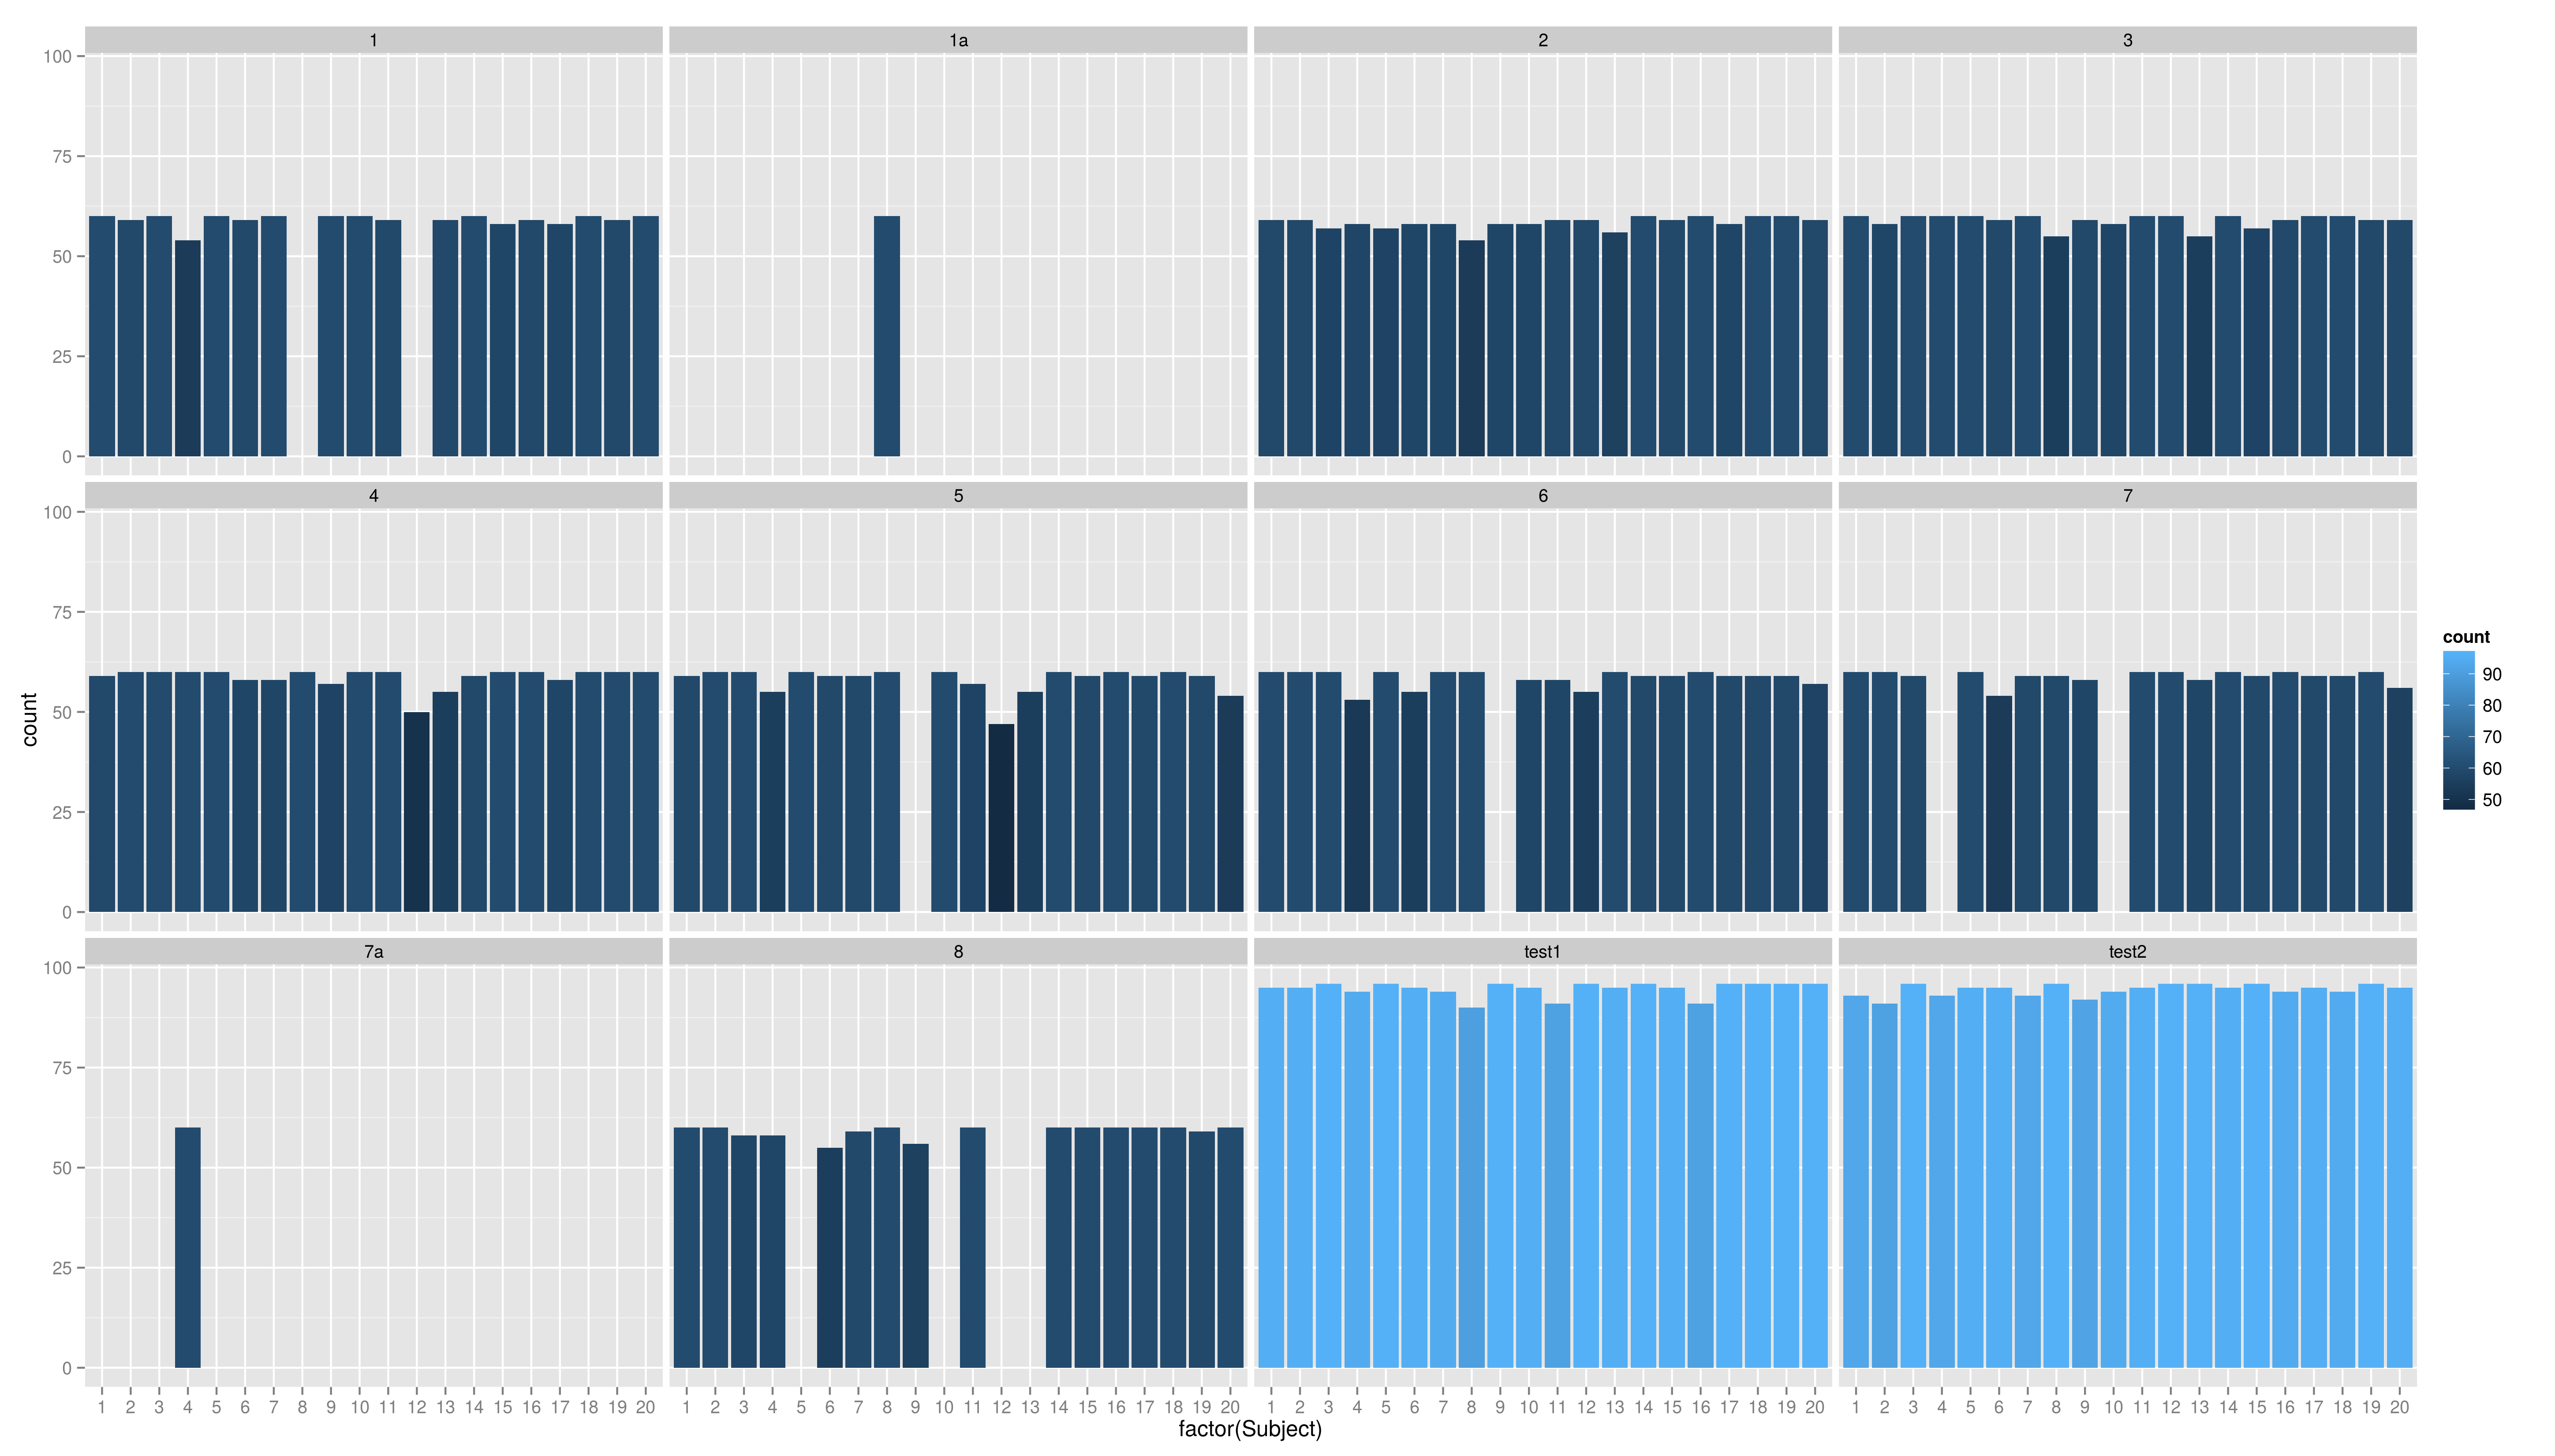
\includegraphics[width=8cm, height=4cm]{graph1.png}}{graph1.png}
\end{center}
\end{frame}

\begin{frame}[fragile]\frametitle{Summary Graphics}
  \begin{itemize}
  \item so there are problems in coding of the test id
  \item we remove the letters at the end using \texttt{str\_replace()}
  \end{itemize}
\begin{exampleblock}{Input/Output}\tiny
\begin{verbatim}
> data$testid <- str_replace(data$testid,"[a-z]$","")
> data$testid <- factor(data$testid,
+                       levels=c("test1","1","2","3","4","5","6","7","8","test2"))
> table(data$Subject,data$testid)
    
     test1  1  2  3  4  5  6  7  8 test2
  1     95 60 59 60 59 59 60 60 60    93
  2     95 59 59 58 60 60 60 60 60    91
  3     96 60 57 60 60 60 60 59 58    96
  4     94 54 58 60 60 55 53 60 58    93
  5     96 60 57 60 60 60 60 60  0    95
  6     95 59 58 59 58 59 55 54 55    95
  7     94 60 58 60 58 59 60 59 59    93
  8     90 60 54 55 60 60 60 59 60    96
  9     96 60 58 59 57  0  0 58 56    92
  10    95 60 58 58 60 60 58  0  0    94
  11    91 59 59 60 60 57 58 60 60    95
...

\end{verbatim}
    \end{exampleblock}
\end{frame}


\begin{frame}[fragile]\frametitle{Summary Graphics}
\begin{exampleblock}{Input/Output}\tiny
\begin{verbatim}
> ggplot(data,aes(x=factor(Subject),fill=..count..)) +
+     geom_bar() +
+     facet_wrap(~testid)
\end{verbatim}
    \end{exampleblock}
\begin{center}
  \linkimage{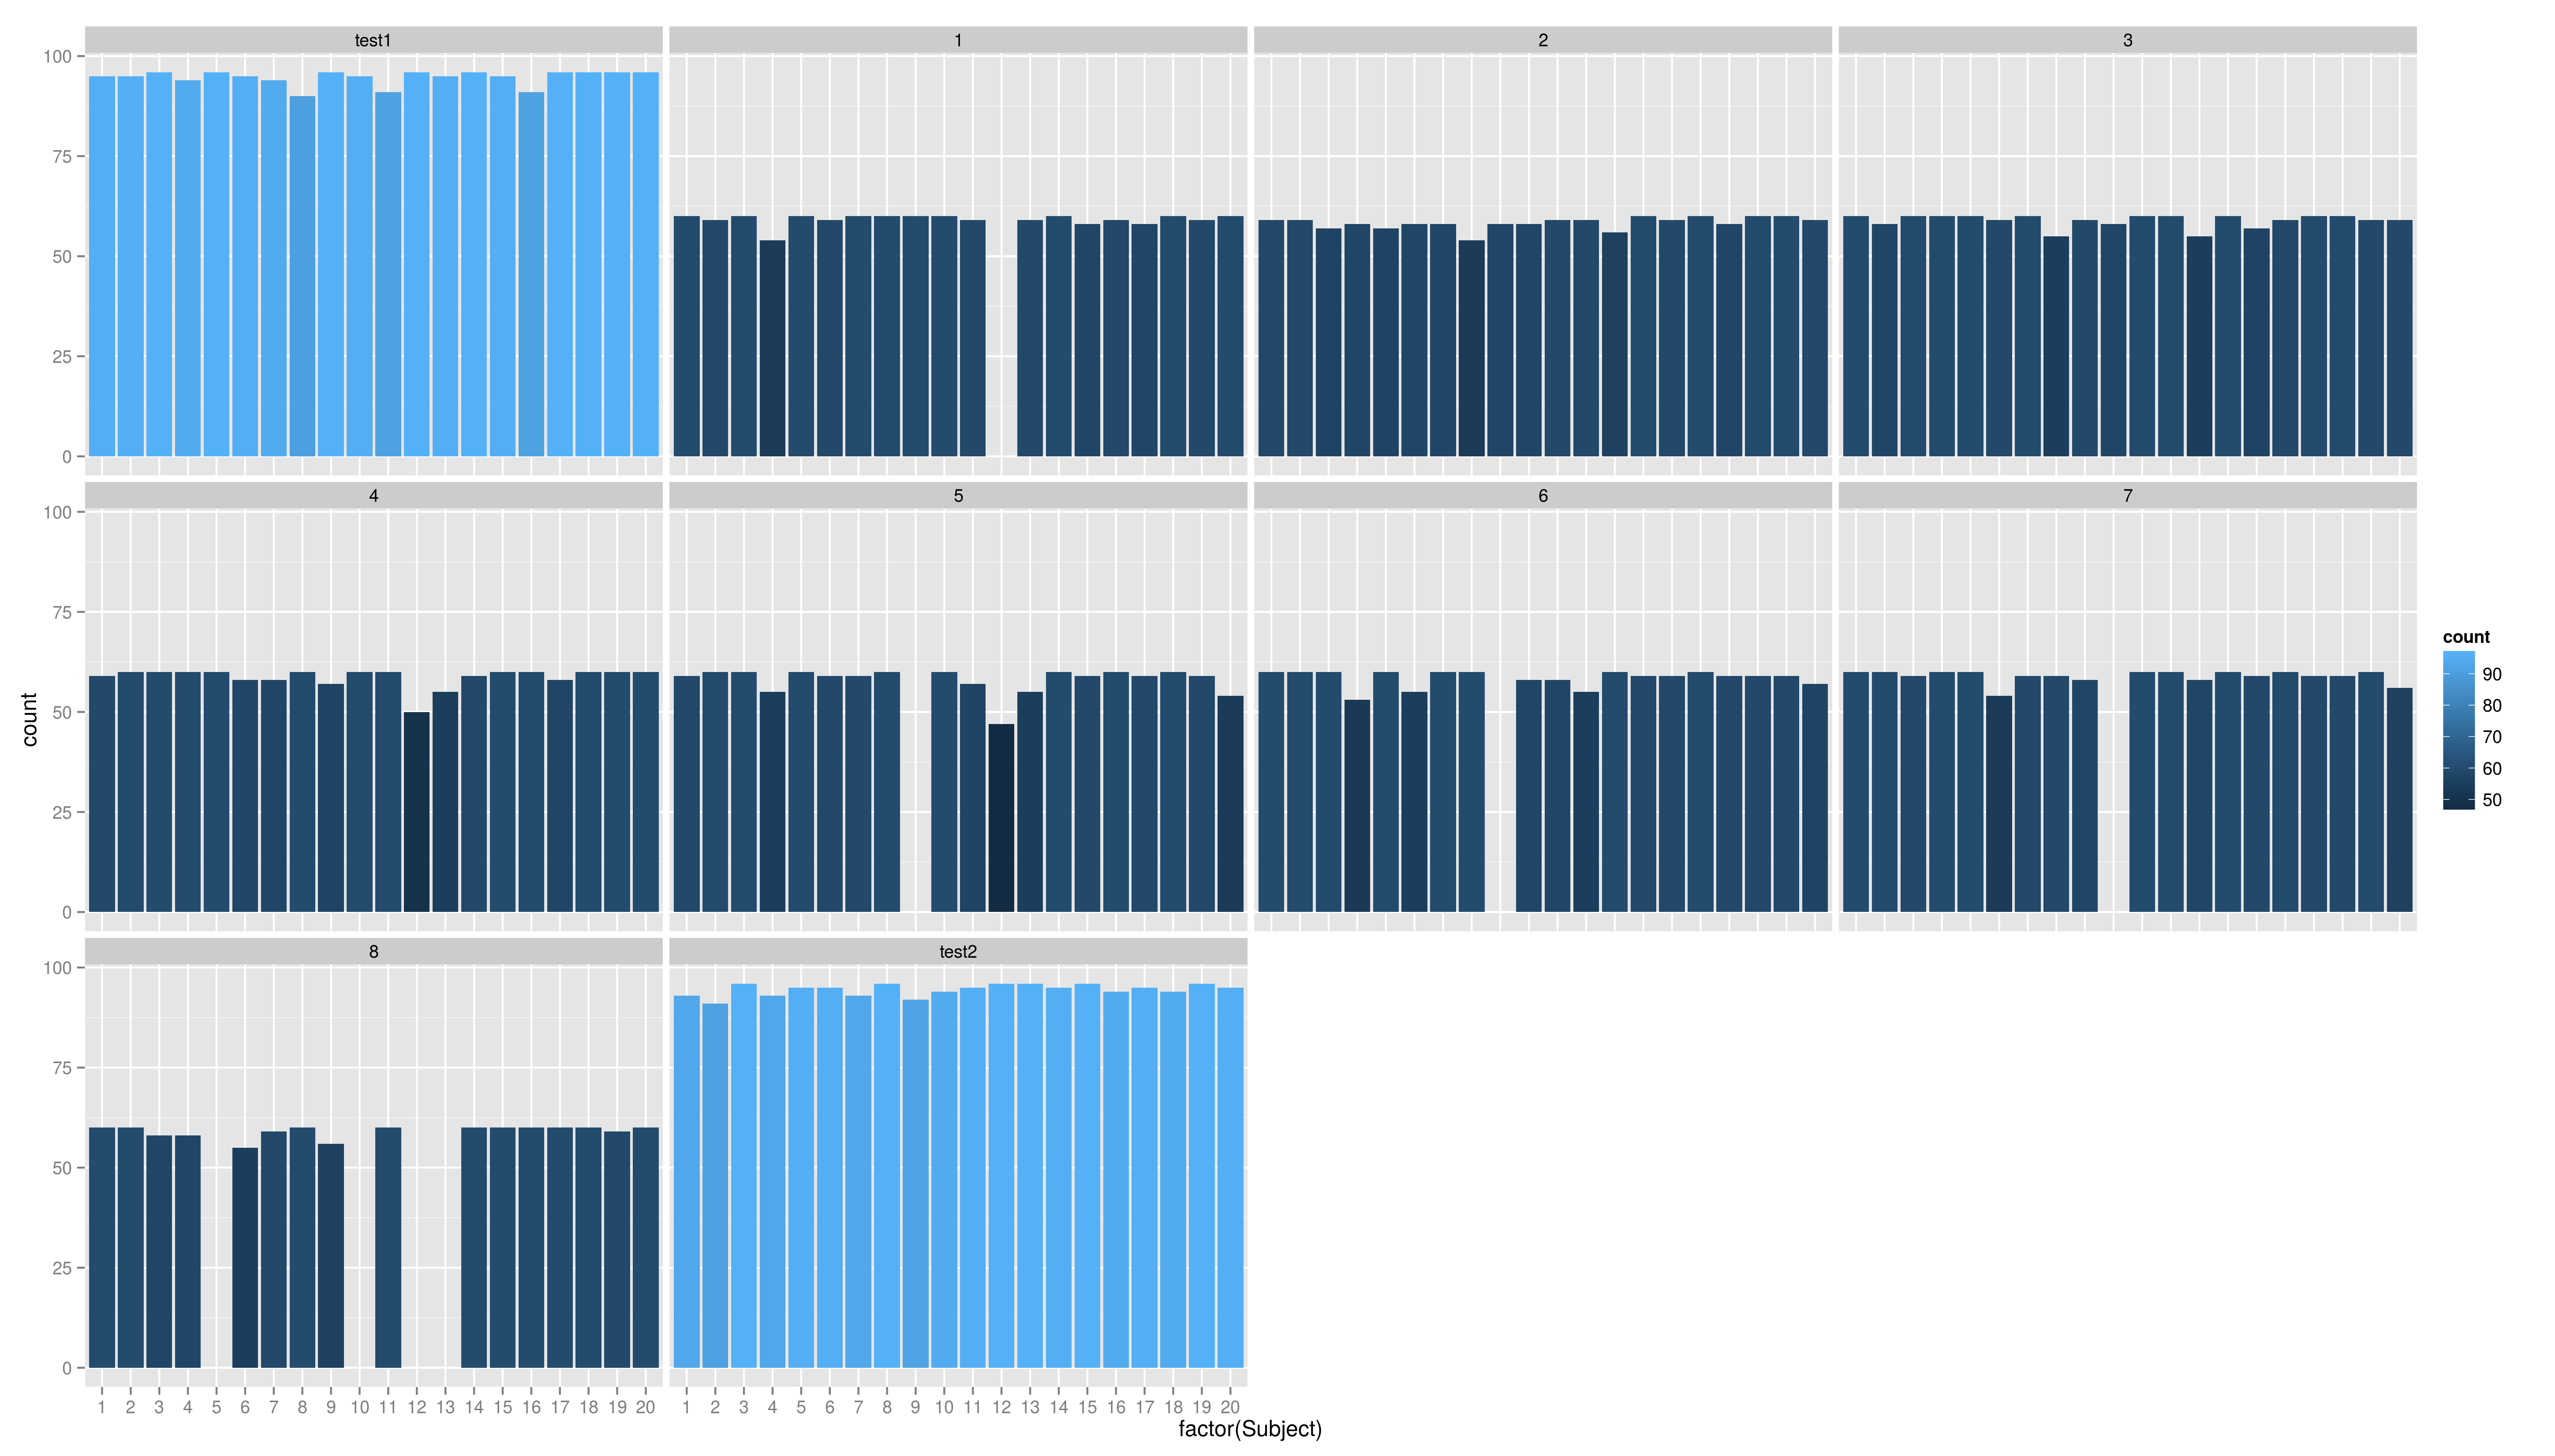
\includegraphics[width=8cm, height=4cm]{graph2.png}}{graph2.png}
\end{center}
\end{frame}

\begin{frame}[fragile]\frametitle{Summary Graphics}
And another one.
\begin{exampleblock}{Input/Output}\tiny
\begin{verbatim}
> ggplot(data,aes(x=testid,fill=Stim.Type)) +
+     geom_bar(position=position_fill()) +
+     facet_wrap(~Subject)
\end{verbatim}
    \end{exampleblock}
\begin{center}
  \linkimage{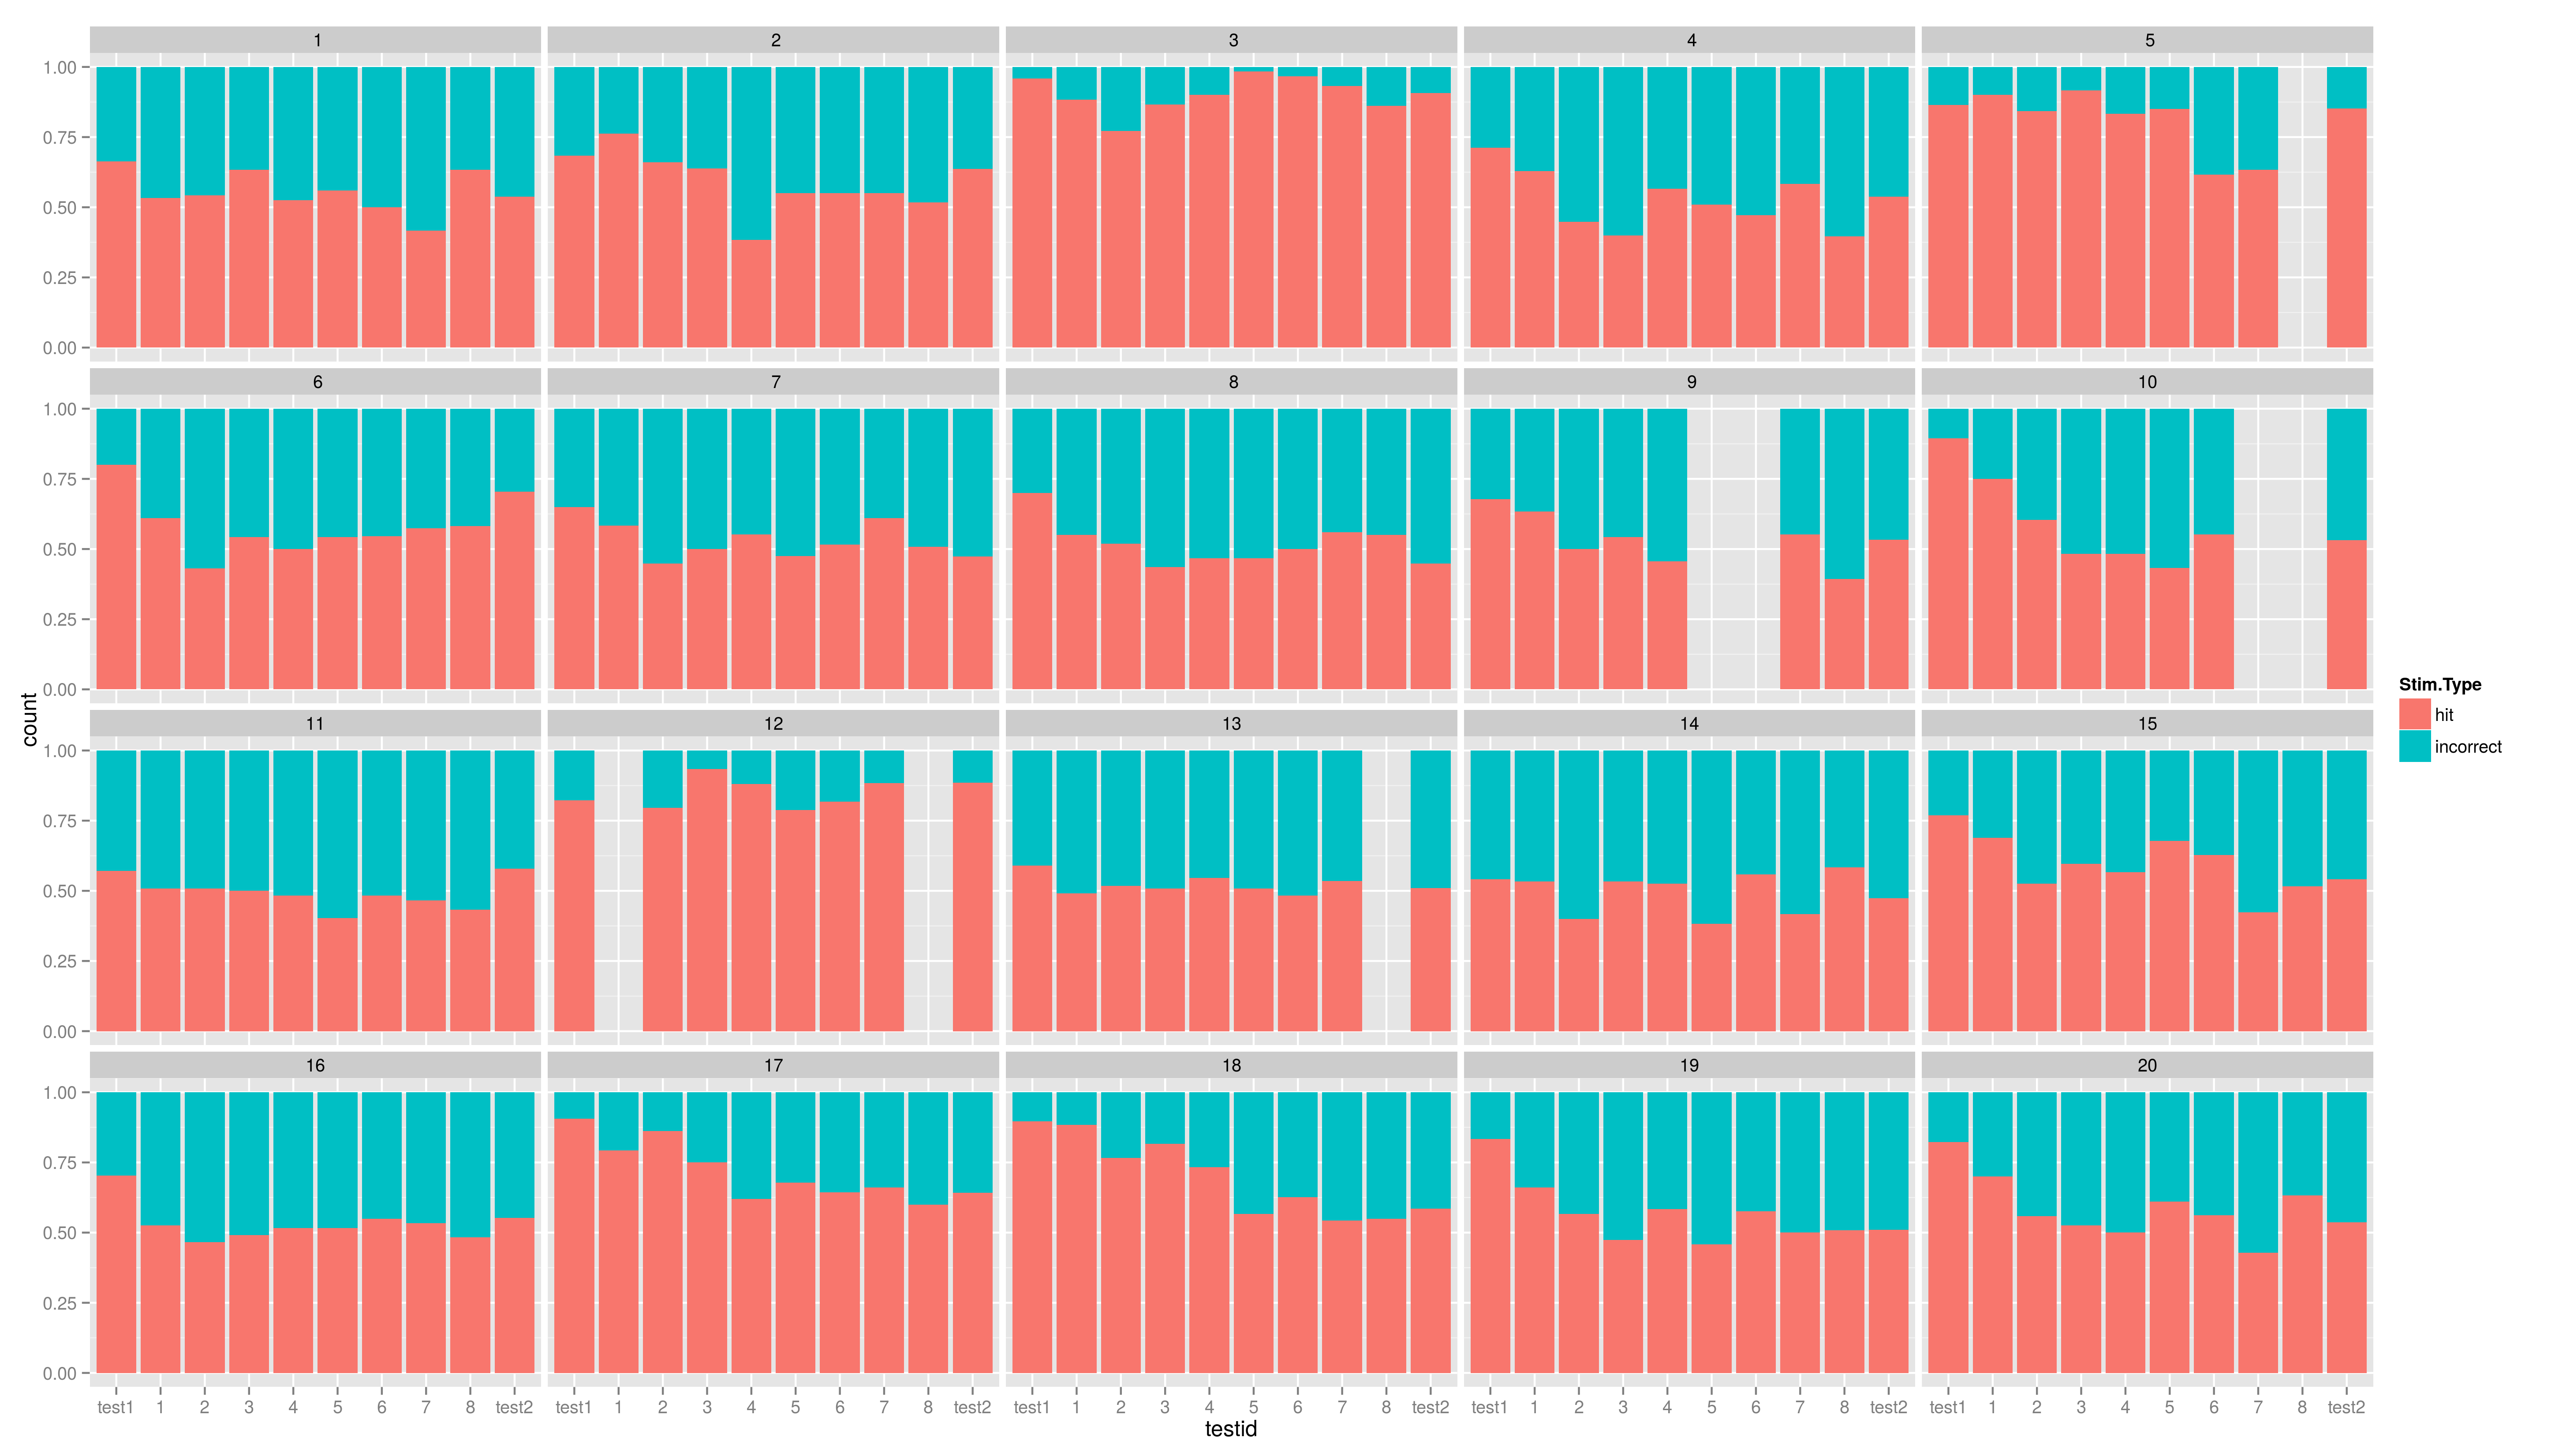
\includegraphics[width=8cm, height=4cm]{graph3.png}}{graph3.png}
\end{center}
\end{frame}



\appendix
\flushlinkimages

\end{document}
